\label{ch:design}

\section{Bottom-up Abstraction}
\label{sec:bottom-up}
When developing a property set for the AHB system bottom-up, abstraction is a priority. The entire RTL model is therefore ideally verified in a single cluster. 
It is on the other hand not feasible to represent this multi-master design without separating the master agents into their own clusters. The reason for this is 
parallelism and the exponential growth in possible states it brings forth. Every master agent acts with independence between idle and request. This means that the properties must capture all possibilities of each input notify signals and requests in every property, which is not feasible already with two master agents.
\begin{wrapfigure}[14]{l}{8cm}
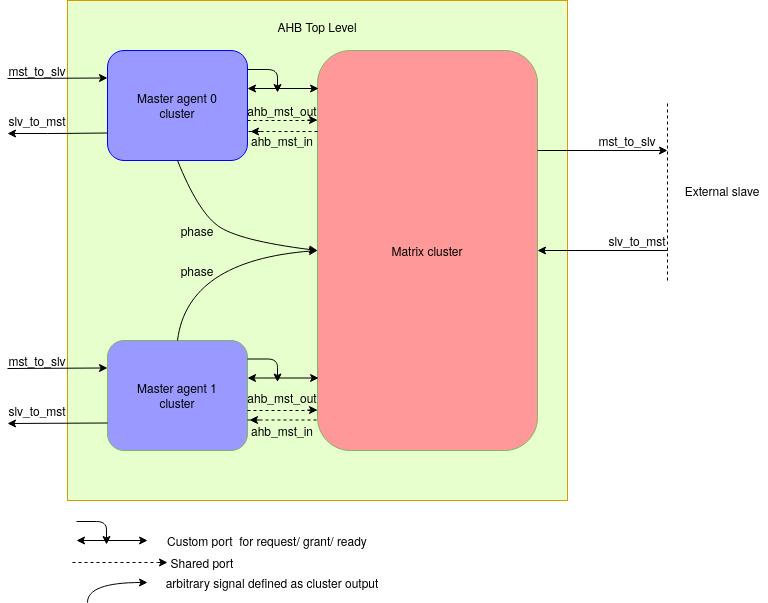
\includegraphics[width=8cm]{figs/Verif/Verif_block.png}
\caption{Verification clusters}\label{fig:verif-clust}
\end{wrapfigure} 

Fig.~\ref{fig:verif-clust} provides an overview of the verification clusters and their connections. I/O connections are listed with their compound names with port type indicated in the legend. The master agent is a relatively simple design so this section is mainly focused on the matrix cluster. The Gap Free Verification process introduced in Sec.~\ref{sub:gfv} is carried out on the matrix cluster. \par
It is not possible to determine every state of the matrix cluster by observing internal registers alone. There are no registers differentiating between a default master being idle or in the data phase of a transfer. Looking at signal values in the past require constraints on wait states. A better alternative is to define the state of the default master agent as an output to its cluster and an input to the matrix cluster. The states are determined based on this signal, address and data bus ownership as well as slave notify signals. The minimum Conceptual State Machine is listed below, possible transitions are indicated by numbering. 
\begin{enumerate}
 \item Idle: No transfer in progress, \textbf{HREADY} is set and bus is ready to accept a new request (1,2).
 \item Address: A transfer is initiated, \textbf{HREADY} is set and bus is ready to accept a new request.(3)
 \item Slave(x)\_write: Important state for each slave output. (4)
 \item Slave(x)\_read: Important state for each slave input (5)
 \item Data\_end: A transfer is completed, \textbf{HREADY} is set and bus is ready to accept a new request. (1,2,3) 
\end{enumerate}

Operation properties must cover all possible requests, read and write transaction to all slaves, success and error response from slaves as well a transaction to the default slave. Most properties have a duration of one, with write transactions, error response from slave and default slave response as exceptions, which lasts two time points. 

Registers in the arbiter RTL module store the address and data bus ownerships in \textit{master\_sel} and \textit{r\_master\_sel} respectively. The address and data bus signals are multiplexed master agent outputs, with selection based on bus ownership. Because they are not outputs of registers within the design, issues occur with determining the signals at time \ITLKW{t}+1 based on signals at time \ITLKW{t} when the ownership returns to the default master. Default values can be assigned to the visible register macros to counteract this issue, see Sec.~\ref{sec:refine} for specifics. \par
The remaining determination requirements are signal outputs. Slave notify signals and \textbf{HREADY} must be determined at all times. Slave outputs need only be determined when their associated notify is set. \textbf{HGRANTx} must be determined whenever \textbf{HREADY} is set, whereas \textbf{HRESP} and \textbf{HRDATA} need only be determined when a slave responds. It is currently not feasible to represent this in the ESL model, so all master agent outputs are determined when \textbf{HREADY} is set. \par
\textbf{HGRANTx} is not a register output which entails that it may change its value before the clock edge. This causes problems with the generated properties, since a request at time \ITLKW{t} is granted at time \ITLKW{t}. This signal must be determined as the output of a function, which is described in Sec.~\ref{sec:refine}. Something to note on the other agent outputs; their values are dependent on which slave is selected, this complicates determination so default values of zero are assigned in the slave agents after each transfer. \par
This section has described the essentials for proving completeness on the matrix cluster for single transfers. Extended functionality such as burst transfers are briefly discussed in Sec.~\ref{sec:burst}
 

\section{ESL}
After a complete set of abstract properties for the bus matrix is derived, the ESL model is developed. In the previous section it was established that master agents must be verified in a separate cluster. This translates to the ESL by separating the master agents in their own SystemC-PPA. Defining a suitable interface between the master agent and bus matrix require careful consideration. \par
With blocking ports, correct simulation behavior and the highest level of abstraction is achieved, but that creates an issue with the bus matrix ESL module for multiple masters. Up to three blocking ports need to be serviced in the same time-point due to parallelism, which is not implemented in SystemC-PPA. A helper module is introduced which is not intended for property generation, but to serve as an emulated port interface. The requirements of this module is described in Sec.~\ref{sub:portem}.

\subsection{Bus matrix}
No more than three explicit states are required to model the bus matrix at the ESL. The communication with the emulated port signals each of these important states in the generated properties. The implementation of the bus matrix ESL covered in Sec.~\ref{sub:bus-matrix} is elaborated with requirements and options. \par
\textit{update\_requests} is required to be a non-blocking write in each state. It must be a write to unconditionally hand over control to the emulated port, so that master agents can advance their state machine in synchronization with the bus matrix. It must always be non-blocking because no wait property can be proven in either of the three states. \par
All master agent interfaces are represented with shared ports, which are directly connected between the agents and the bus matrix in the top-level module. Only the response payloads can be routed through the emulated port, which provide little benefit. It is not done in this work to keep the dependencies on the helper module to a minimum. Before each interaction with the emulated port, either the response payload or default values must be assigned all master agent ports. \par
If there are no pending requests when the bus transitions from \textit{Address} state or \textit{Data} state, default values must be assigned to the variables storing address and control signals. When the bus transitions from $Address\rightarrow Data$ and it is a write transaction, it is best to fetch the payload from that master agent again. Otherwise the properties prove that data is sampled in the address phase, which makes the system dependent on its own weakness. If the transaction is a read, the data part of the payload must be zeroed, or wrong values are reflected in the properties. \par
\WKSAY{Im having a hard time figuring out what to write here} 
 

\subsection{Master Agent}
  
\subsection{Emulated port}
\label{sub:portem}
The emulated port has strict requirements to ensure correct simulation behavior, both in terms of synchronization and in terms of arbitration. This module can not be proven formally to be a sound abstraction of the RTL for the same reason that it is implemented. The chosen arbitration scheme must be manually verified to exactly match the arbitration scheme in the bus matrix. \par
The port must wait for a synchronization signal from the bus matrix, perform request forwarding, service all applicable blocking ports and return to wait for a synchronization signal without interruption. This is accomplished by utilizing blocking inputs for both ports from each master agent, and performing a non-blocking read, only if there is a writer waiting. 


\section{Refining the Properties}
\label{sec:refine}
This section describes how the generated property sets are refined to hold on the design. Every I/O signal, visible register and important state is represented with a macro, which is of the form \par  
\ITLKW{macro} signal\_name : \ITLIW{type} := refinement \ITLKW{end macro}; \par
Every blocking port in the SystemC-PPA has signal macros for the payload, as well as a set of macros, sync and notify, which represent the wait(event) and event notify respectively. Before covering the individual clusters property refinement, the emulated port interfaces will be explained collectively. \par
The emulated port interfaces exclusively use the sync and notify to convey information. Some of these do not exist in the RTL design, so they are given abstract values to satisfy the properties. Following is a pseudo refinement of the existing signals, with a two master system as example. \par
\ITLKW{macro} agent0\_request\_notify : \ITLIW{boolean} := hbusreq0 \ITLKW{end macro}; \\
\ITLKW{macro} update\_requests\_sync : \ITLIW{boolean} := hbusreq0 \ITLRW{or} hbusreq1 \ITLKW{end macro}; \par
\ITLKW{macro} agent0\_request\_sync : \ITLIW{boolean} := hgrant0 \ITLRW{and} hready0 \ITLKW{end macro}; \\
\ITLKW{macro} agent0\_ready\_sync : \ITLIW{boolean} := hready0 \ITLKW{end macro}; \\
\ITLKW{macro} update\_requests\_notify : \ITLIW{boolean} := \\ hready0 \ITLRW{and} hready1 \ITLRW{or} \\ hgrant0 \ITLRW{and} hready0 \ITLRW{or} \\ hgrant1 \ITLRW{and} hready1 \\ \ITLKW{end macro}; \par
This covers the complete top-level connection of all the signals, as long as this behavior is guaranteed within the emulated port it should not leave a gap in verification. However, this representation is not sufficient to use in the completeness description to determine hbusreqx as input, or hgrantx as output. The macros generated from the shared interfaces are used in the completeness description for these two signals in addition. 

\subsection{bus matrix}

All remaining I/O signals are refined with the similarly named top-level signal, where next(hwdata) is used to capture that data is sampled in the data phase. The exceptions are hwrite and hsize and hgrant, which are represented at the ESL using enum values. The first two are conditionally refined with the top-level signals as follows.\\   
\ITLKW{macro} agent0\_sig\_hwrite : \ITLIW{mask} := \ITLKW{if}(agent0.hwrite = \ITLRW{"000"}) \ITLKW{then} MT\_B ...\par
The refinement of hgrant require an added macro which serves as a function to determine its value at any given time. The \ITLIW{type} of hgrant is redefined from mx\_grant to \ITLIW{boolean}. The default master is granted when no other master holds a grant. Every master which is not default master is refined as follows: \\
\ITLKW{if}(hready \ITLRW{and} hbusreqx \ITLRW{and} \ITLRW{not(}higher\_request\ITLRW{)}) \ITLKW{then true}\\
\ITLKW{elsif}(addr\_own = x \ITLRW{and not(}hready\ITLKW{)}) \ITLKW{then true \\else false}  \par
The only visible registers extracted from the ESL model are the address and control signals, address bus ownership and state variables. The data bus variable is optimized away from the SystemC-PPA, which is not ideal as we need this register to determine the states. A macro for the data bus ownership and the default master state is added to the description. The address and control signals are refned with the address mux outputs in the arbiter module, if there is an agent with a transfer in the address phase, otherwise they are given the same default values as in the ESL. This can be determined by checking if the default master state is address, or the address bus ownership not equal to zero. Recall that master zero is default master in this work. \par
The visible registers extracted from the state variable of the ESL model, are not represented anywhere in the RTL. There are no state variable called phases so an unused type "\textit{phases}" is added to the RTL so that these visible registers can be mapped. \par
The state macros representing the state of communication with slaves are simply refined with their associated notify signal. The remaining states are refined as follows: 
\begin{itemize}
 \item Idle: If default master is not in the state Address or Data, but still owns both address and data bus, the bus is idle.
 \item Address: If default master owns the data bus, but is not in the data phase, and the default master is in the address phase or does not own the address bus, the bus is in state Address. 
 \item Data\_end: update\_requests\_notify is set, default master is in the data phase or does not own the data bus.  
\end{itemize}

Finally, all properties which end with an error signal or starts with a write request on the address bus must be refined so \ITLKW{t\_end}=\ITLKW{t}+2.

\subsection{Master Agent}
only a few words here, the assertion. 

\section{RTL}
The open source architecture used in this work is defined in one architectural module, in the file \textit{ahb\_arbiter.vhd}. It uses arbitration functions from the file \textit{ahb\_func.vhd}, slave address configurations from \textit{ahb\_configure.vhdl}, packages from \textit{ahb\_package.vhd} and components from \textit{ahb\_component.vhdl}. \par
All payloads visible from the top-level in the ESL design are added to the package file, together with state machine declarations for the master and slave agent, as well as the unused type representing the ESL states of the bus matrix. It also containts some constants to offer readability for the signals which are hardwired. \par
Component declaration of all system modules are added to the component file, this includes agents, arbiter and bus matrix. The bus matrix is a top-level module for the arbiter, which instantiates the arbiter and provides default master selection and master priority. Master zero is highest priority, which decreases with incrementing numbers. For simplicity, the highest priority master is set as the default in this work. \par
The configuration file contains the slave address ranges in decimal number, as well as the remapped address ranges of the slaves. Remap is not implemented in this work so they must be equal, remap is hardwired to zero for extra security. \par
The top-level module must include the following: \par
\ITLKW{library} \ITLIW{ieee}; \\
\ITLKW{use} \ITLIW{ieee}.\ITLIW{logic\_1164}.\ITLKW{all}; \\ 
\ITLKW{use} \ITLIW{ieee}.\ITLIW{numeric\_std}.\ITLKW{all}; \\
\ITLKW{use} \ITLIW{work}.ahb\_package.\ITLKW{all}; \\
\ITLKW{use} \ITLIW{work}.ahb\_components.\ITLKW{all}; \par
The arbiters reset is active low, so the top-level reset must be inverted before assigning it to the matrix port map. All slave agents require their address offset as a generic in the form of a 32-bit logic vector. All master and slave agents are connected to their inputs and outputs of the matrix with corresponding numbers. 

\subsection{Slave Agent}
The slave agent includes the same packages as the top-level, except for the components. It includes an additional package \ITLIW{ieee}.\ITLIW{std\_logic\_unsigned}.\ITLKW{all} so that the slave address offset can be subtracted from the haddr input. \par
It is important that all output signals are register outputs, where hready is an exception, this should be controlled as a combinational output: \\
hready <= '1' \ITLKW{when} section = idle \ITLKW{else} '0'; \par
The module has a combinational state machine, which use flags to signal when address/control and data gets clocked in. When response data is written to the outputs, a flag is set which is used together with hready to signal when the default values are assigned.

\subsection{Master Agent}

 

\section{Building the Generator}
The generator consists of two parts; the hardware generator and the plugin which generates and refines the property sets. The hardware generator takes number of masters and slaves as input arguments and reads a textfile of slave address ranges which are stored in a map. The generator instantiates two classes with this data which together generate the system at the RTL and ESL. The generator produces a textfile with the same stored data, converted for use within the plugin. It continues to call the plugin with the bus matrix and master agent SystemC-PPAs in turn. The plugin reads the text file and distinguishes between the two SystemC-PPAs to generate a refined property set and completeness description for each. 

\subsection{Hardware generator}
The generator uses the slave input argument to decide how many lines of the address map text file to read. It recognizes the words "start" and "end" to determine the start and end of the range. A separate map is produced for the ESL and RTL generation to avoid the need to convert the address format on the fly. The classes which generate the ESL and RTL are so similar in structure and function that they will not be described separately. \par
A set of files are generated for each abstraction layer, which are files that are not static with respect to number of masters and slaves. All files such as agents, dummies for testbench and arbiter remain in the output folder untouched and must not be deleted or modified. \par
All files are generated with an output filestream which is assigned a function output. Each file has its own dedicated function which write the module description to a local stringstream. Each function uses the stored number of masters, slaves and address map to produce its module according to the requested configuration. 

\subsection{Plugin: PrintAHB}
The plugin starts by reading the plugin data text file, which contain number of masters and slaves, as well as slave address ranges. The slave address ranges were used in an earlier implementation, but are not removed from the plugin data in case they are needed in the future. The plugin checks if the file name if it is the bus matrix or master agent and calls the appropriate function to generate the property files. 
\subsubsection{Bus matrix}



\section{Simulation}



\section{Experimental Results}
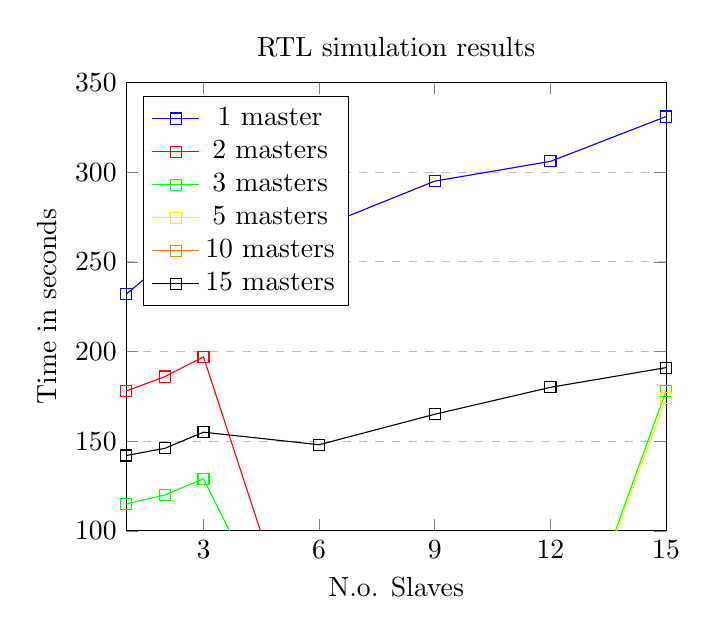
\begin{tikzpicture}
\begin{axis}[
    title={RTL simulation results},
    xlabel={N.o. Slaves},
    ylabel={Time in seconds},
    xmin=1, xmax=15,
    ymin=100, ymax=350,
    xtick={0,3,6,9,12,15},
    ytick={100,150,200,250,300,350},
    legend pos=north west,
    ymajorgrids=true,
    grid style=dashed,
]
\addplot[
    color=blue,
    mark=square,
    ]
    coordinates {
    (1,232)(2,250)(3,257)(6,269)(9,295)(12,306)(15,331)

    };
    \addlegendentry{1 master}

\addplot[
    color=red,
    mark=square,
    ]
    coordinates {
    (1,178)(2,186)(3,197)(6,0)(9,0)(12,0)(15,0)
    };
    \addlegendentry{2 masters}

\addplot[
    color=green,
    mark=square,
    ]
    coordinates {
    (1,115)(2,120)(3,129)(6,0)(9,0)(12,0)(15,178)
    };
    \addlegendentry{3 masters}

\addplot[
    color=yellow,
    mark=square,
    ]
    coordinates {
   (1,0)(2,0)(3,0)(6,0)(9,0)(12,0)(15,174)
    };
    \addlegendentry{5 masters}

\addplot[
    color=orange,
    mark=square,
    ]
    coordinates {
    (1,0)(2,0)(3,0)(6,0)(9,0)(12,0)(15,0)
    };
    \addlegendentry{10 masters}

\addplot[
    color=black,
    mark=square,
    ]
    coordinates {
    (1,142)(2,146)(3,155)(6,148)(9,165)(12,180)(15,191)
    };
    \addlegendentry{15 masters}
    
\end{axis}
\end{tikzpicture}


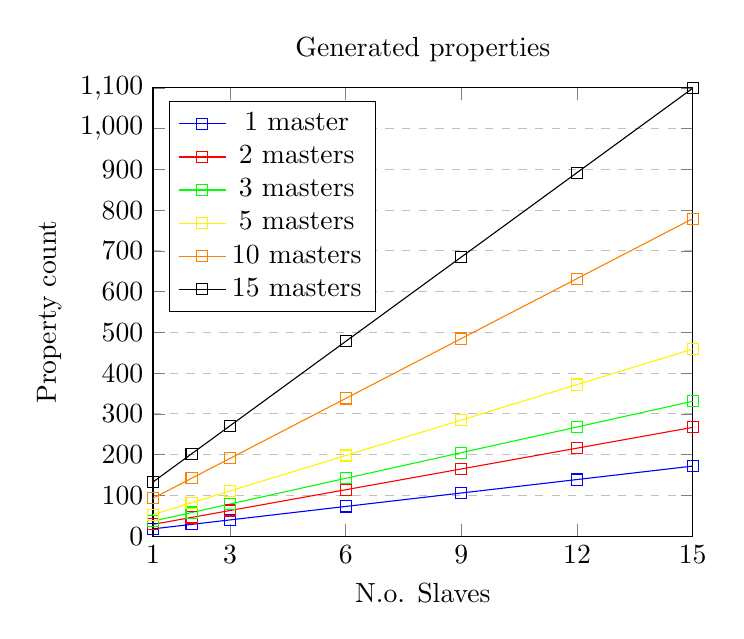
\begin{tikzpicture}
\begin{axis}[
    title={Generated properties},
    xlabel={N.o. Slaves},
    ylabel={Property count},
    xmin=1, xmax=15,
    ymin=0, ymax=1100,
    xtick={1,3,6,9,12,15},
    ytick={0,100,200,300,400,500,600,700, 800, 900, 1000, 1100},
    legend pos=north west,
    ymajorgrids=true,
    grid style=dashed,
]
\addplot[
    color=blue,
    mark=square,
    ]
    coordinates {
    (1,18)(2,29)(3,40)(6,73)(9,106)(12,139)(15,172)

    };
    \addlegendentry{1 master}

\addplot[
    color=red,
    mark=square,
    ]
    coordinates {
    (1,29)(2,46)(3,63)(6,114)(9,165)(12,216)(15,267)
    };
    \addlegendentry{2 masters}

\addplot[
    color=green,
    mark=square,
    ]
    coordinates {
    (1,37)(2,58)(3,79)(6,142)(9,205)(12,268)(15,331)
    };
    \addlegendentry{3 masters}

\addplot[
    color=yellow,
    mark=square,
    ]
    coordinates {
   (1,53)(2,82)(3,111)(6,198)(9,285)(12,372)(15,459)
    };
    \addlegendentry{5 masters}

\addplot[
    color=orange,
    mark=square,
    ]
    coordinates {
    (1,93)(2,142)(3,191)(6,338)(9,485)(12,632)(15,779)
    };
    \addlegendentry{10 masters}

\addplot[
    color=black,
    mark=square,
    ]
    coordinates {
    (1,133)(2,202)(3,271)(6,478)(9,685)(12,892)(15,1099)
    };
    \addlegendentry{15 masters}
    
\end{axis}
\end{tikzpicture}




\section{Concept: Burst Transfers}
\label{sec:burst}
